\section{Mini-MAC}
\label{mini-mac}


%The best solution, in that it is implementable and does not change the network infrastructure, to preventing replay and masquerade attacks on the CAN bus to this point is the work presented in Lin-MAC. The underlying MAC protocol was not described, however, and as the ECUs on this node are time-, memory-, and processing power-constrained, some testing must be done to determine which construction is the most suitable for the environment. HMAC is by far the most famous and most popular MAC construction, so three variants of HMAC (that is, HMAC with three underlying keyed-hash functions) were selected for consideration for this project. HMAC is widely used for two key reasons. 1) The security of HMAC is mathematically related to the security of the underlying hash function, which makes it relatively easy to trust and 2) it is extremely easy to plug in various hash functions, making it easy to update to a new implementation if issues are found in the currently used hash\cite{HMAC}\cite{FIPS-198-1}. They are implemented in C on the MSP430.

%The equation for calculating the HMAC is as follows: 

%$$ \text{HMAC} = H((K_0\oplus \text{opad})\vee H((K_0\oplus \text{ipad})\vee \text{message}) $$

%Where $K_0$ represents the key, which is sized depending on the underlying hash, and opad and ipad are the outer and inner hash padding strings respectively. These strings are constant strings represented by 0x5C and 0x36 repeated until the hash input string is of the appropriate size. The term $H$ represents the hash function used to generate the HMAC. \cite{FIPS-198-1}

%Figure 1 depicts the key group key distribution model used for Mini-MAC. Note that as multiple ECUs share the same key, messages may be sent to multiple nodes without re-calculating a new MAC for each recipient. This is a key bus overhead reduction compared to Lin-MAC.
	
%	\begin{figure}
%		\centering
%		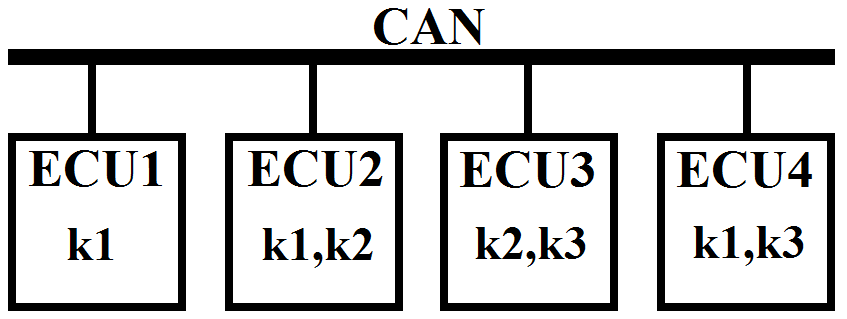
\includegraphics[width=\columnwidth]{figures/key_distribution.png}
%		\caption{Mini-MAC Key Distribution}
%	\end{figure}

Mini-MAC can be broken into three conceptual tiers--archictecture, design and implementation. This section describes Mini-MAC at each of these levels. The architecture describes the high-level critical points that differentiate Mini-MAC from other MAC protocols, while the design level describes the algorithm used to generate the resulting MAC. Finally, this section describes how Mini-MAC is implemented with various hash functions.

While a MAC such as HMAC will defeat a masquerade attack, it will not be able to defeat a replay attack, as the previously recorded message will have a valid MAC. To address this, some time-based token, frequently a counter, can be added to the computation of the MAC. The resulting tag is unique to the message and the time it is sent, which prevents an illegitimate node from simply replaying a message seen in the past.

For the automotive environment, the time-based HMAC has one significant downside - the size of packets on the CAN bus is very small (64B) and the size of the HMAC bit string is, depending on the hash function used, at least twice that size. In order to use normal HMAC, bus traffic would go up some large factor determined by the size of the hash used. 

Mini-MAC is a variable-length Message Authentication Code protocol based on HMAC. It selects an output size to match the available space in a given CAN message. It uses secret keys as well as variable-length counters to seed and condition the HMAC to guarantee against repeated MACs.

The core principle of Mini-MAC is that in the automotive environment attackers have a small window of time to break the network. With that in mind, it is possible to design a security mechanism that is capable of defending the network on that very short scale of time without breaking real-time or processing capability constraints.

\subsection{Architecture}

%Mini-MAC uses group-shared keys (Figure 2) instead of pairwise keys. The use of group keys means that a message need be sent only once and the entire group which needs the message can verify the sender rather than having a separate MAC sent for each recipient. This means Mini-MAC does not need to send any additional  messages in order to provide authentication, which meets the design requirement for bus traffic overhead. Group key distribution is possible because at the time of system design the engineers know exactly which ECUs will need to communicate with which others. There does not need to be a dynamic group update function as there are no circumstances in which a group should change.

There are four key points that help define Mini-MAC:
\begin{itemize}
\item Variable-size output to fit the CAN packet
\item Group-shared keys
\item A split counter used for MAC seeding and truncation
\item Message history to confuse MAC output.
\end{itemize}

\textcolor{red}{Note: Do you like the itemization of these points, or would it be better organized in a paragraph?}

Mini-MAC uses group-shared keys (Figure 2) instead of pairwise keys. For example, the group comprised of ECUs 1, 2, and 4 share key 1. The use of group keys means that a message need be sent only once and the entire group which needs the message can verify the sender rather than having a separate MAC sent for each recipient. This means Mini-MAC does not need to send any additional message in order to provide authentication, which meets the design requirements for bus traffic overhead. Group key distribution is possible because at the time of system design the engineers know exactly which ECUs will need to communicate with which others. There does not need to be a dynamic group update function as there are no circumstances in which a group should change.

The downside of using group keys is that if one member becomes compromised, that member has the ability to send illegitimate messages to every other member of the group rather than just one other node as would be the case in a pair-wise key distribution. The choice to use a group key distribution was made for Mini-MAC because security must be balanced with efficiency, and the bus traffic increase resulting from pair-wise key distribution may be too high to meet real-time constraints. There may be many groups composed of only two nodes, in which case security is not reduced at all compared to a pair-wise protocol.

A split counter is used to alter and select the final MAC from the HMAC. The low-order bits are used to seed the HMAC, while the high-order bits are used to select the starting bit in the HMAC from which the Mini-MAC is drawn.

Message traffic history is used as a post-HMAC confusion step -- the previous messages sent on the sender's ID are used to change the resulting HMAC. This prevents the same MAC being used after the counters roll over. Unless the same message (or message pattern) is repeated exactly, the same MAC will not be issued, even on identical counter values.
	
	\begin{figure}
		\centering
		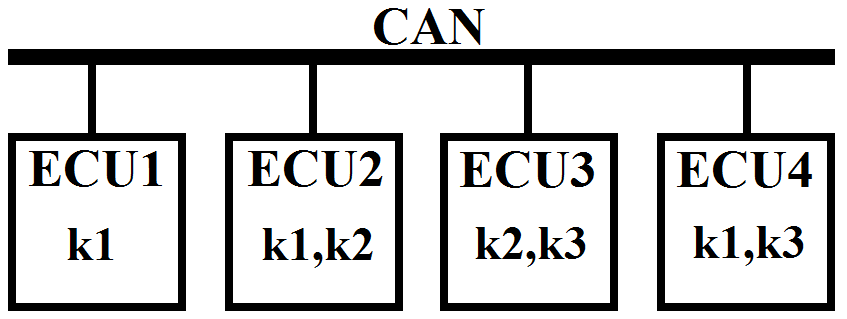
\includegraphics[width=\columnwidth]{figures/key_distribution.png}
		\caption{Mini-MAC Key Distribution}
	\end{figure}
	
	
\subsection{Design}
%\textcolor{red}{Note: I don't have a solution to dealing with faults at this time. I believe there are some good ideas in previous work that I will take another look at\\Update: The previous work tends not to mention dealing with faults. In similar systems, there is a mechanism for setting counters to specific values on a fault, which should allow re-sync between sender and recipient. In practice, end users more commonly reset counters to 0 and start from the beginning. Even though this is less secure the procedure is more simple. I'm not sure how I want to address it. Do you have any thoughts?}

%\textcolor{red}{Note: I don't have the figure we put together on the board in CDL the other day done. All I have is a trackpad now, when I track down a proper mouse I will put it together and add it, as well as references to it throughout the text\\ I'm going to re-write this entire subsection when I finish that diagram. It's still hard to understand.}

\textcolor{red}{Note: Is this a better way of incorporating the equations into the text?\\ I don't like the figure -- do you have a recommendation for software to create good-looking figures? I've just been using MS Paint and would like to tidy up a few things before submitting.}

One of the most important aspects of HMAC is that it allows the use of a wide range of iterative hash functions as its base. Mini-MAC, being based on HMAC itself, similarly allows various hash functions as a base.

	\begin{figure}
		\centering
		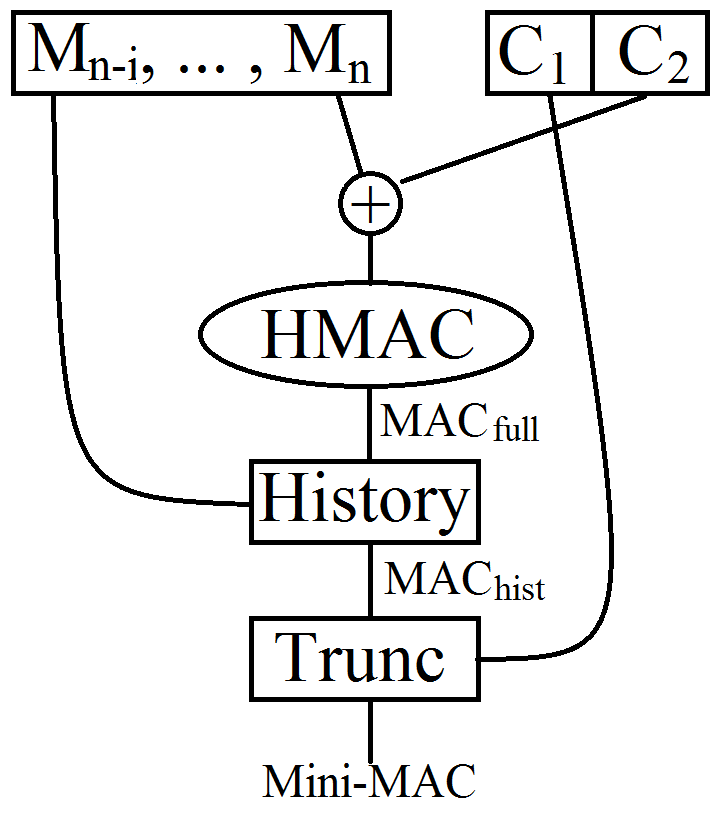
\includegraphics[width=\columnwidth]{figures/minimac_diagram.png}
		\caption{Mini-MAC Construction Diagram}
	\end{figure}

%The calculation of Mini-MAC is only slightly more involved than in the HMAC construction---before computing the HMAC, the input is XORed with a counter, and after the HMAC is computed the result is XORed with previous messages and trimmed.

The computation of the Mini-MAC begins with the creation of an input string, 

\begin{equation}
\text{Input} = \text{Message}_n\oplus\text{Counter}_{\text{msg}}
\end{equation}

which is used to generate an HMAC value. The HMAC calculation 

\begin{equation}
\text{MAC}_{\text{full}} = \text{HMAC}(\text{Input})
\end{equation}

results in a full-size MAC without any message history input. For $h$ = the number of messages in history to use, 

\begin{equation}
\text{For }i=1:h\text{, MAC}_\text{hist} = \text{MAC}_{\text{full}}\oplus\text{Message}_{n-i}
\end{equation}

where $\text{MAC}_\text{hist}$ is a full-size MAC with added message history information. This value is finally truncated according to the trunc function, defined as

\begin{equation}
\text{MAC}_{\text{mini}} = \text{MAC}_{\text{full}}(l,l+s)
\end{equation}

where $l$ is the rollover counter, which ticks when the message counter rolls over, and $s$ is the available size in the CAN message for the Mini-MAC. The result of the two-counter system is that a new MAC is generated for each value of the message counter, and from that MAC, the bits starting with the bit addressed by the rollover counter are taken as the Mini-MAC. This way, when the message counter rolls over, the bit start location shifts so the same Mini-MAC is not re-used until the rollover counter rolls over.



%The full construction protocol is shown below in Equation 2 through Equation 5, where $n$ is the number of the message in a sequence of messages, $n=0$ being the most recent message, $h$ is the number of messages from history to be used for MAC confusion, $l$ the starting bit to select the Mini-MAC from within the full-size MAC, and $s$ being the size of the Mini-MAC in bits. 

%The value of $l$ is determined by a second counter designated the rollover counter, which ticks when the message counter rolls over. The result of this two-counter system is that a new MAC is generated for each value of the message counter, and from that MAC, the bits starting with the bit addressed by the rollover counter are taken as the Mini-MAC. This way, when the message counter rolls over, the bit start location shifts so the same Mini-MAC is not re-used until the rollover counter rolls over.

%\begin{equation}
%\text{MAC}_{\text{mini}} = \text{MAC}_{\text{full}}[l:l+s]
%\end{equation}

%Equation 2 is a simple XOR operation of the message to be sent and the message counter. Equation 3 takes the result of Equation 2 and performs the HMAC on it as detailed in Equation 1. The HMAC is then XORed with previous messages, up to $h$ messages in history, as shown in Equation 4. Finally, in Equation 5, the variable size Mini-MAC is extracted from the full-size, history-based MAC computed in Equation 4.

\subsection{Implementation}
Mini-MAC was implemented with three hash functions--MD5, SHA1, and SHA2. The varying performance and security characteristics of these hash functions provide end users with a spectrum of solutions to choose from without needing to vary the Mini-MAC computation.

\textbf{HMAC-MD5}
We adapted Peslyak's implementation of MD5 for the MSP430 platform. MD5 produces a 128-bit output from a variable length message. Since 2004, the security of MD5 has been severely compromised \cite{Wang-MD5} -- however, tests showed that it was the fastest HMAC construction and for that reason only it was used as a basis for Mini-MAC. It should be noted that any other hash function could be used, but the test was interested in computation speed more than any other metric\cite{MD5}
%The MD5 implementation tested for this project was originally written by Alexander Peslyak \cite{Peslyak} and adapted for the MSP430 platform by the authors. \\-------\\
%Alexander Peslyak \cite{Peslyak} wrote the original MD5 implementation used in this project, and it has been adapted for use on the MSP430 platform by the authors. 
%\textcolor{red}{Note: Which of the above two sounds better? I can change the SHA1 and SHA2 to match}.

%MD5 produces a 128-bit output value from a variable length message. Since 2004, the security of MD5 has been severely compromised \cite{Wang-MD5} -- however, tests showed that it was the fastest HMAC construction and for that reason only it was used as a basis for Mini-MAC. It should be noted that any other hash function could be used, but the test was interested in computation speed more than any other metric\cite{MD5}.

\textbf{HMAC-SHA1}
%The HMAC-SHA-1 implementation used for this project was originally written by Brad Conte \cite{Conte-SHA1} and adapted for the MSP430 platform by the authors. 
We adapted Brad Conte's SHA-1 implementation for the MSP430 platform \cite{Conte-SHA1}. SHA-1 produces a 160-bit output value from variable length inputs. Similar to MD5, security vulnerabilities have been found in SHA-1 \cite{Wang-SHA1}, but it is still used in many applications and will be for the immediate future\cite{FIPS-180-4}.

\textbf{HMAC-SHA256}
%The HMAC-SHA-256 implementation used in this project was originally written by Brad Conte \cite{Conte-SHA256} and was adapted for the MSP430 platform by the authors. 
We also adapted Brad Conte's SHA-256 implementation for the MSP430 platform \cite{Conte-SHA256}. SHA-256 is a member of the SHA-2 family of hash functions. This family produces fixed length output values from variable length input sequences. SHA-2 is still in use and is recommended by NIST as a secure hash function, but SHA-3 will soon replace it\cite{FIPS-180-4}.